% !TeX root = ../main.tex

\documentclass[../main.tex]{subfiles}
\begin{document}

\section{Tổng quan thiết kế mô hình tháp giải nhiệt}
\label{sec:design_overview}

Mô hình tháp giải nhiệt mini được thiết kế để mô phỏng nguyên lý hoạt động của tháp giải nhiệt công nghiệp trong quy mô phòng thí nghiệm. Hệ thống được tối ưu hóa cho việc nghiên cứu, giảng dạy và kiểm chứng các thuật toán giám sát IoT. Thiết kế đảm bảo khả năng tái hiện chính xác các quá trình truyền nhiệt và truyền khối đặc trưng của tháp giải nhiệt thực tế, đồng thời duy trì tính an toàn và dễ vận hành trong môi trường phòng thí nghiệm.

Mô hình được thiết kế theo nguyên tắc tháp giải nhiệt đối lưu hút với cấu trúc compact, cho phép quan sát trực quan các quá trình trao đổi nhiệt và khối. Các thành phần chính bao gồm thân tháp, hệ thống đệm làm mát, bơm tuần hoàn, quạt hút khí và hệ thống gia nhiệt được tích hợp hài hòa để tạo thành một hệ thống hoàn chỉnh.

\begin{figure}[H]
    \centering
    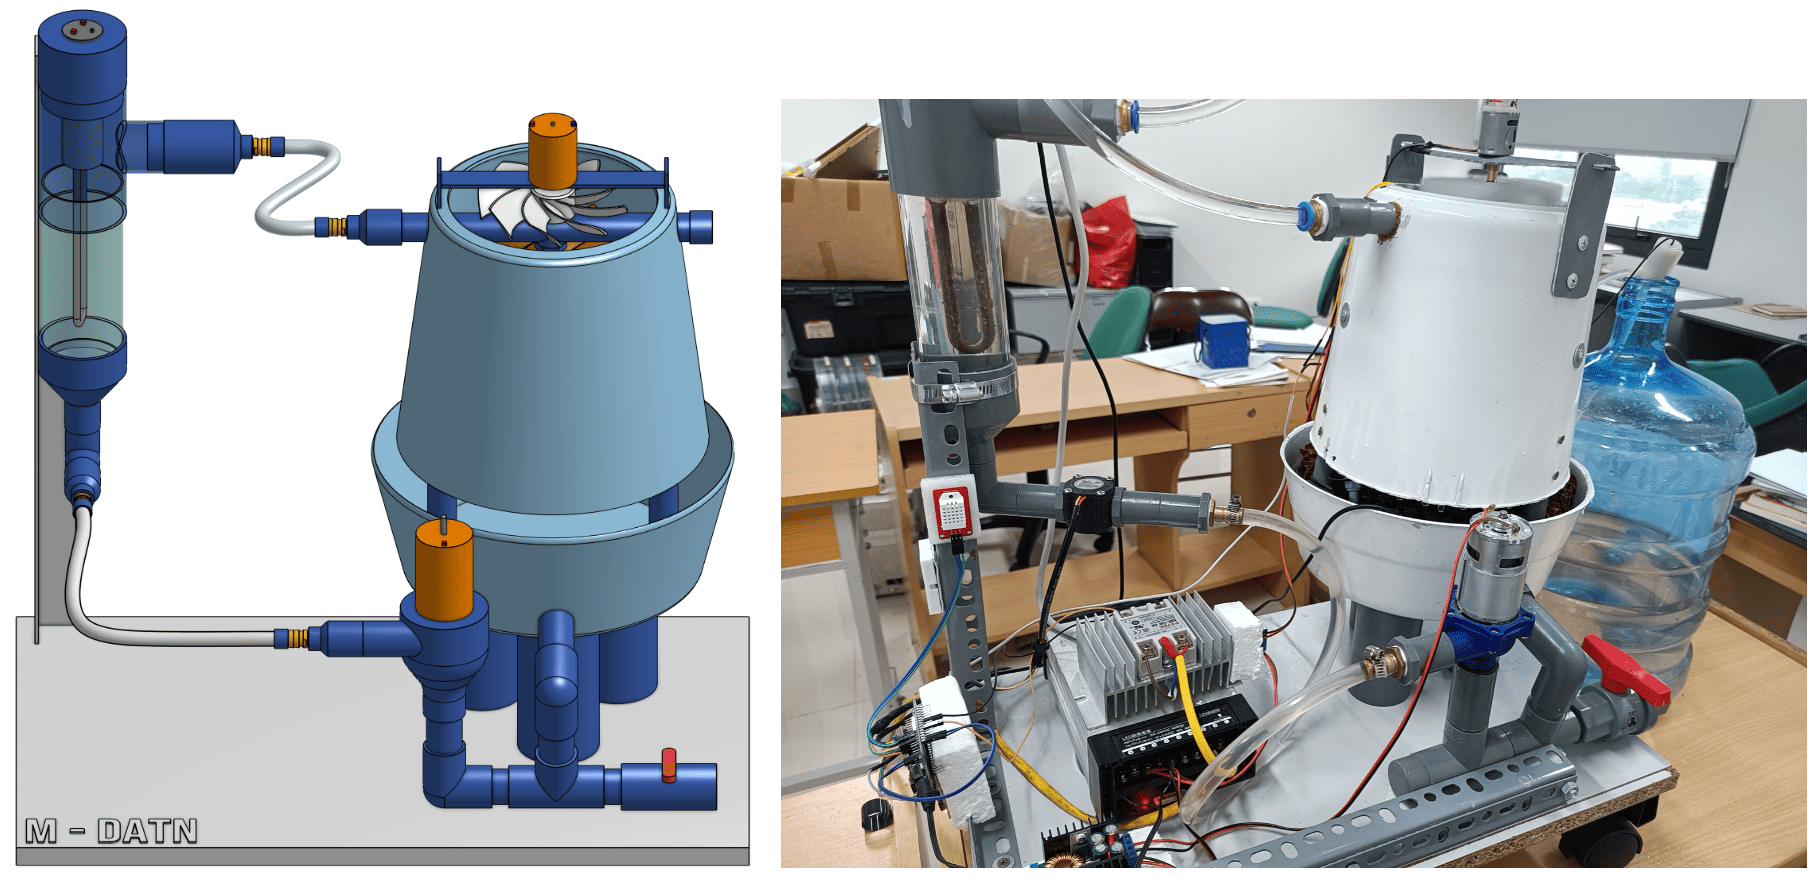
\includegraphics[width=1\textwidth]{Hinhve/thiet_ke_vs_thuc_te.png}
    \caption{Bản vẽ thiết kế mô hình (trái) và mô hình thực tế đã lắp đặt cảm biến (phải)}
    \label{fig:thiet_ke_vs_thuc_te}
\end{figure}

\section{Thông số kỹ thuật chính}
\label{sec:main_specifications}

\subsection{Thông số hình học tháp giải nhiệt}
\label{sec:geometric_parameters}

Thiết kế hình học của mô hình được tối ưu hóa để đảm bảo hiệu suất trao đổi nhiệt tối ưu trong khi duy trì kích thước phù hợp với môi trường phòng thí nghiệm. Tỷ lệ chiều cao/đường kính được thiết kế theo tiêu chuẩn công nghiệp để đảm bảo phân bố đều của dòng khí và nước.

\begin{table}[H]
\centering
\renewcommand{\arraystretch}{1.1}
\caption{Thông số hình học mô hình tháp giải nhiệt}
\label{tab:geometric_specs}
\begin{tabular}{|l|c|c|}
\hline
\textbf{Thông số} & \textbf{Giá trị} & \textbf{Đơn vị} \\
\hline
Chiều cao tổng thể & 492 & mm \\
\hline
Đường kính ngoài thân tháp & 267 & mm \\
\hline
Đường kính trong thân tháp & 230 & mm \\
\hline
Chiều cao vùng đệm làm mát & 40 & mm \\
\hline
Chiều cao vùng phân phối nước & 20 & mm \\
\hline
Chiều cao bể chứa nước & 99 & mm \\
\hline
Diện tích mặt cắt làm việc & 0,053 & m$^2$ \\
\hline
Thể tích làm việc & 9,5 & lít \\
\hline
\end{tabular}
\end{table}

\begin{figure} [H]
    \centering
    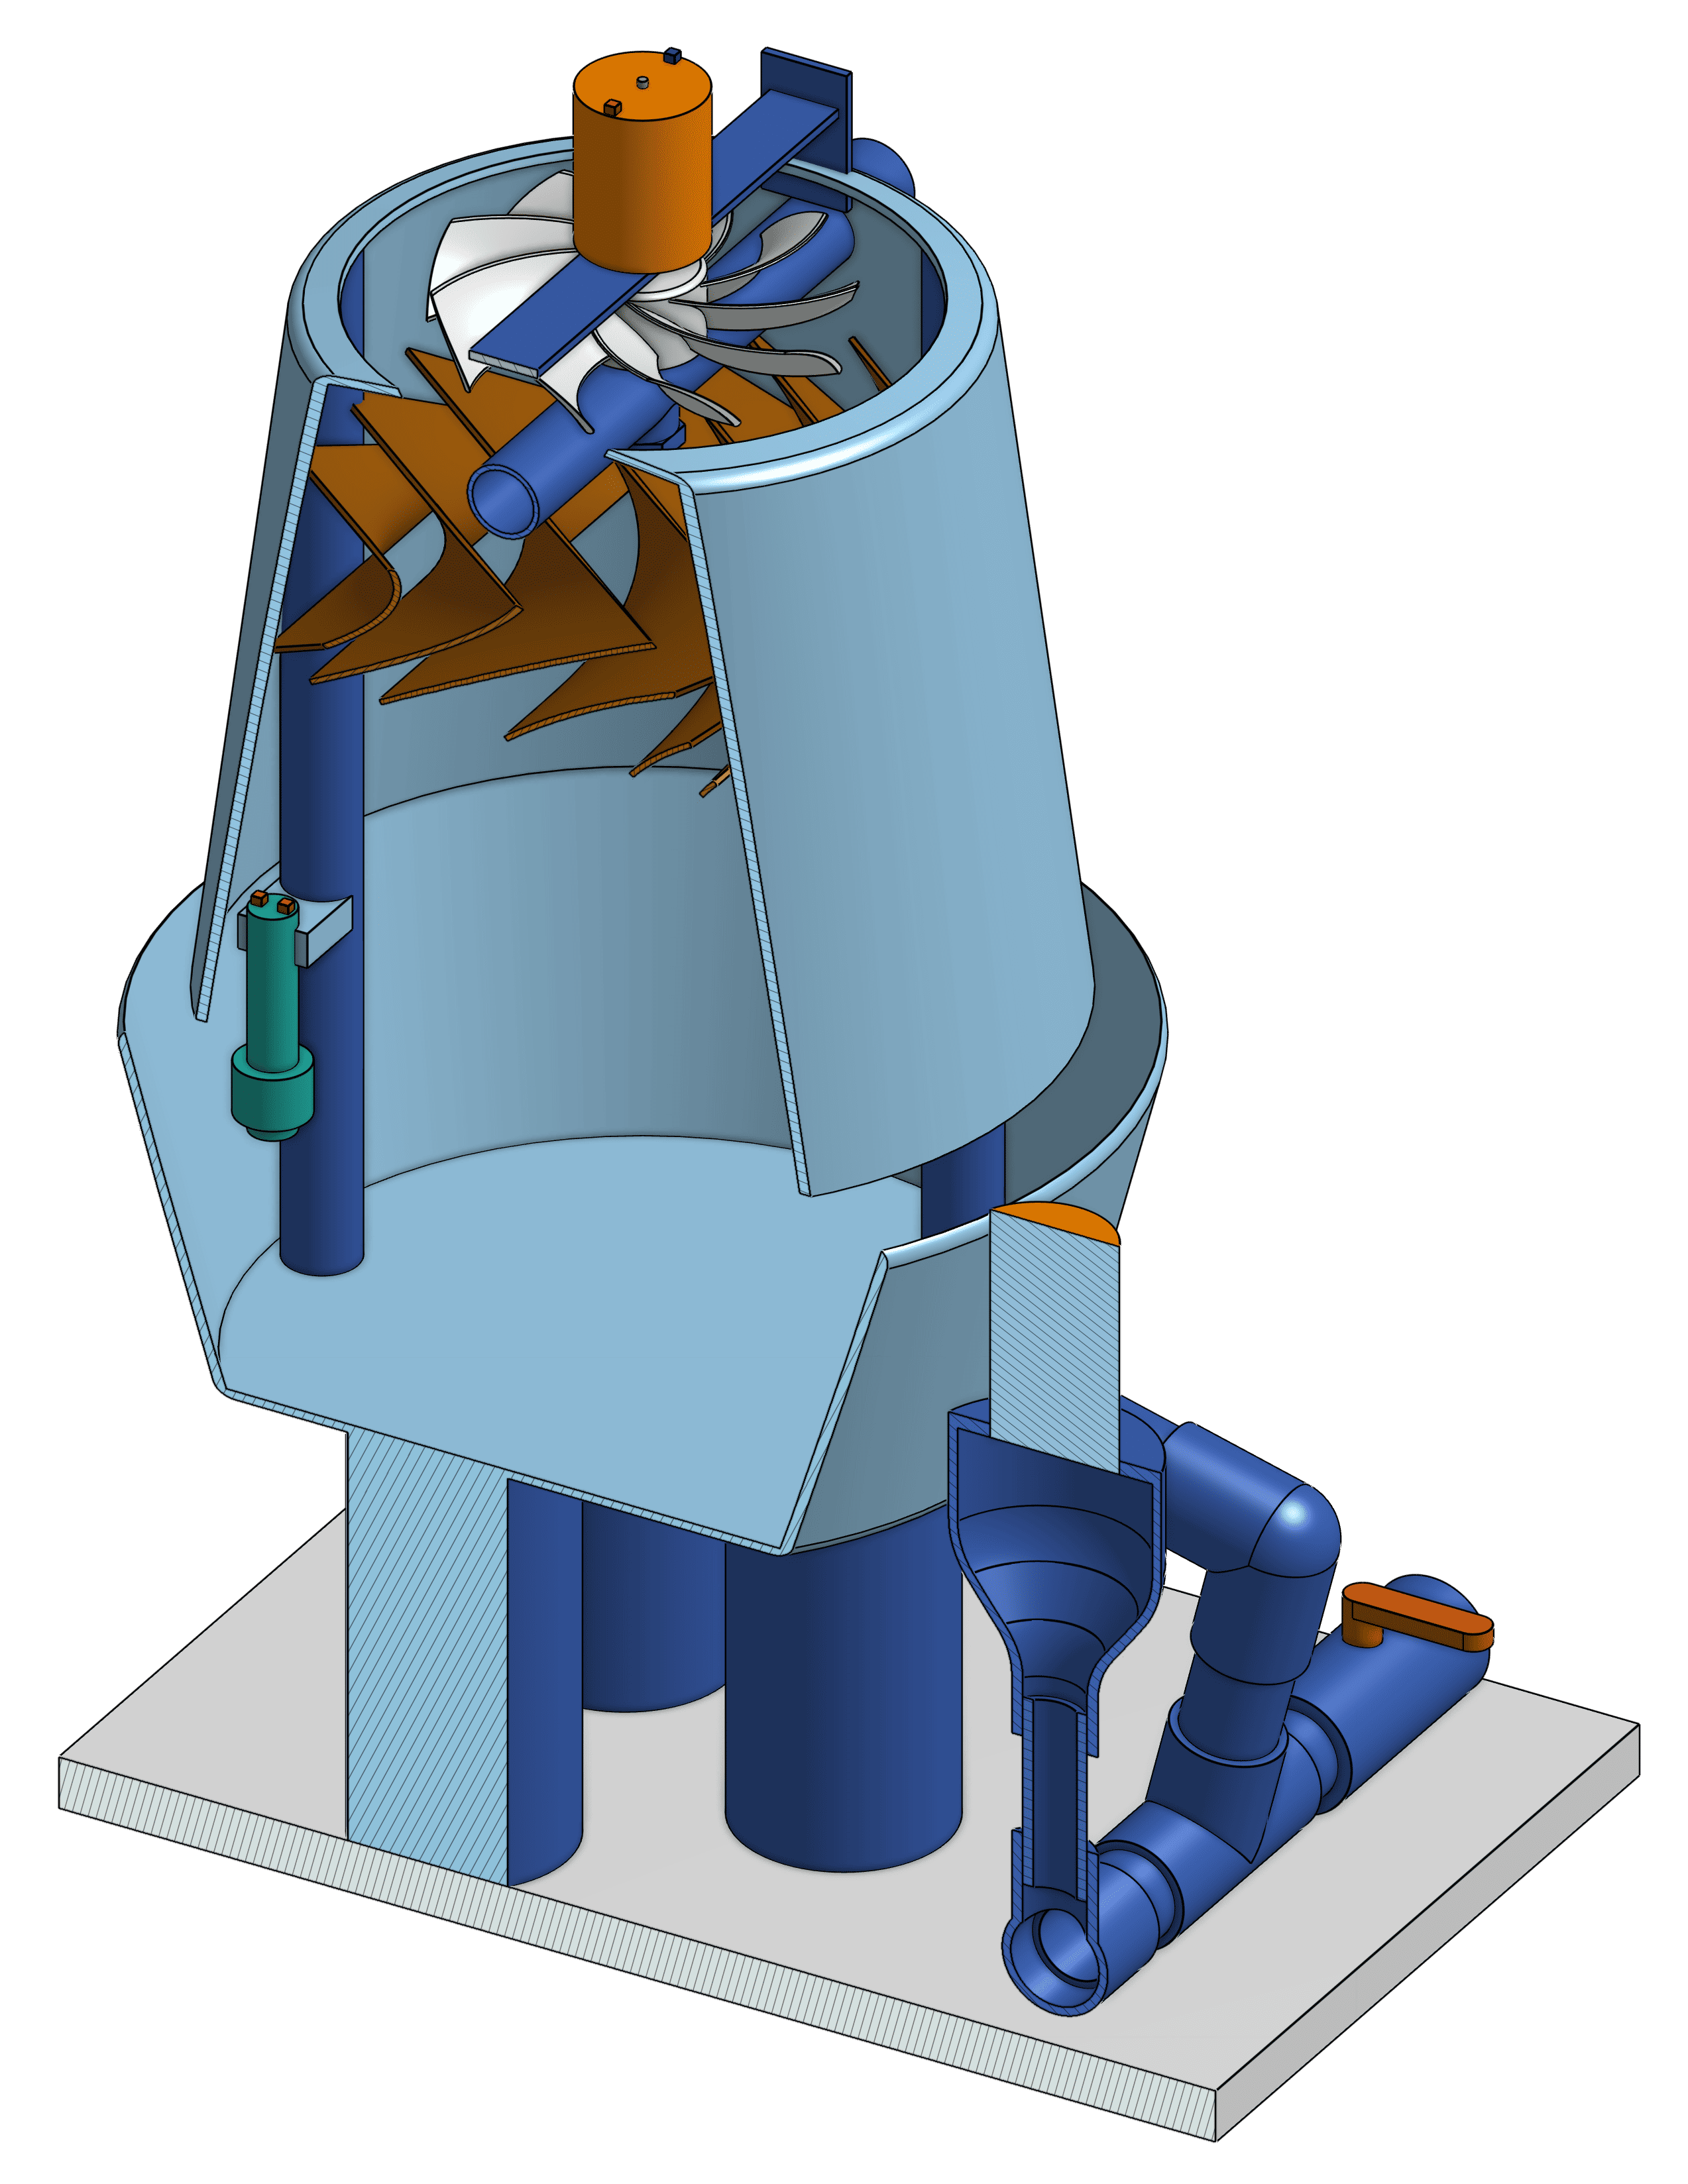
\includegraphics[width=0.6\textwidth]{Hinhve/mat_cat.png}
    \caption{Mặt cắt của mô hình tháp giải nhiệt}
    \label{fig:mat_cat}
\end{figure}

\subsection{Hệ thống đệm làm mát}
\label{sec:fill_system}

Hệ thống đệm làm mát đóng vai trò quan trọng trong việc tăng diện tích tiếp xúc giữa nước và không khí. Thiết kế đệm tổ ong thông minh được lựa chọn để tối ưu hóa hiệu suất trao đổi nhiệt và giảm thiểu tổn thất áp suất.

\begin{figure} [H]
    \centering
    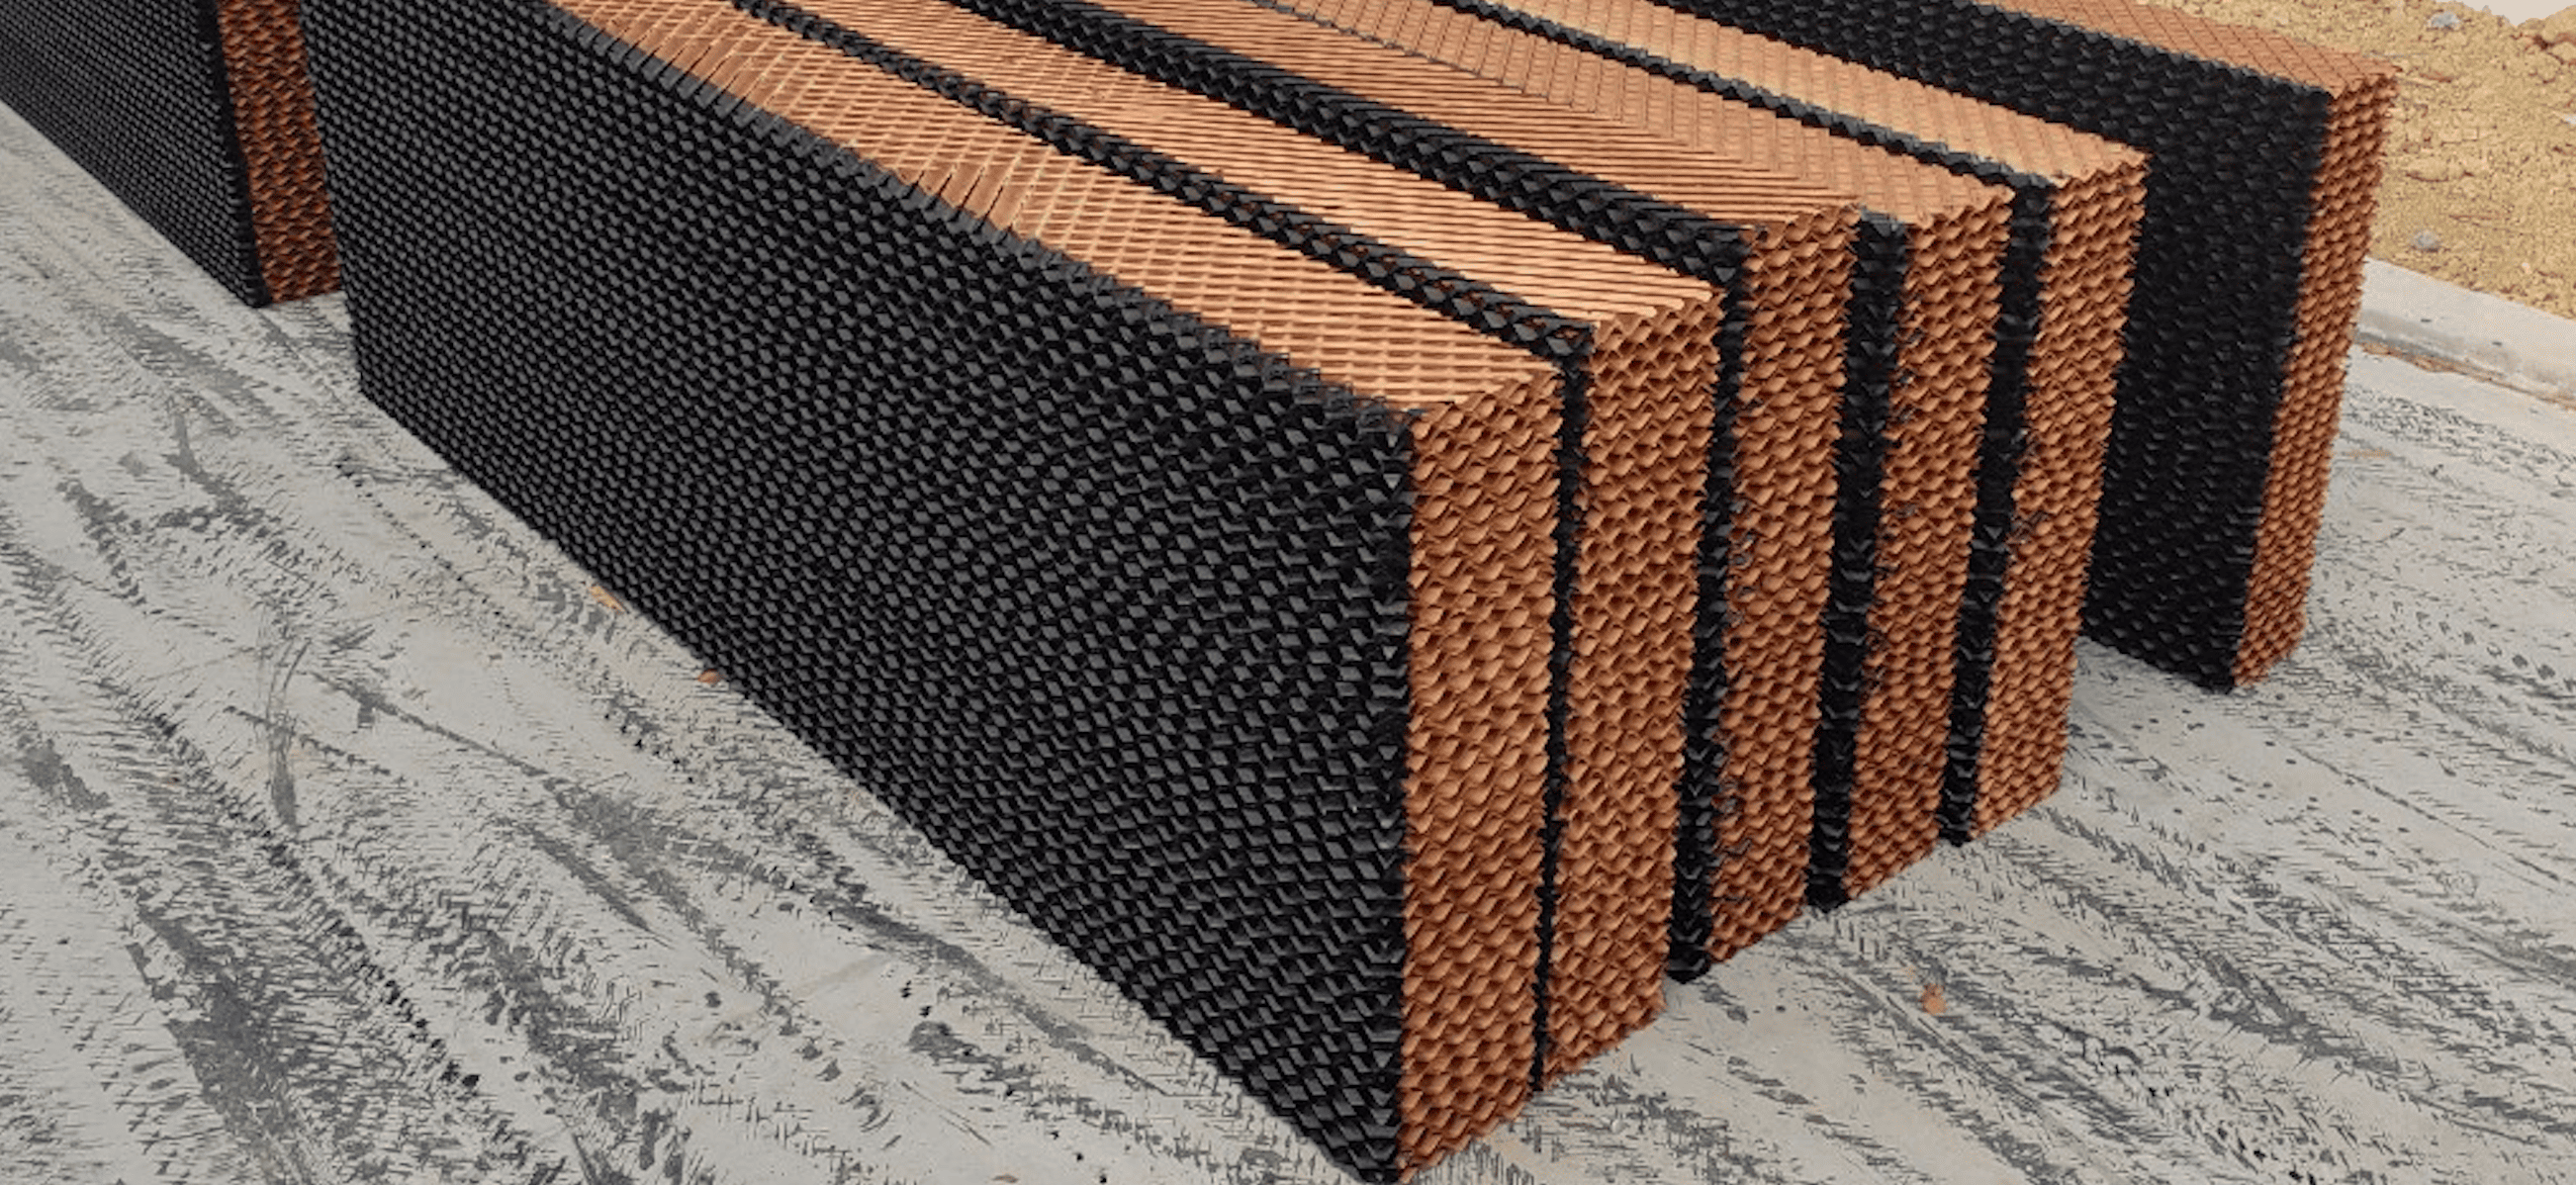
\includegraphics[width=1\textwidth]{Hinhve/cooling_pad.png}
    \caption{Đệm làm mát kiểu tổ ong}
    \label{fig:de_mat}
\end{figure}

\begin{table}[H]
\centering
\renewcommand{\arraystretch}{1.1}
\caption{Thông số hệ thống đệm làm mát}
\label{tab:fill_specs}
\begin{tabular}{|l|c|c|}
\hline
\textbf{Thông số} & \textbf{Giá trị} & \textbf{Đơn vị} \\
\hline
Vật liệu đệm & Giấy cellulose cao cấp & - \\
\hline
Thiết kế đệm & Tổ ong thông minh & - \\
\hline
Độ dày đệm & 40 & mm \\
\hline
Số tầng đệm & 1 & tầng \\
\hline
Diện tích tiếp xúc riêng & 285 & m²/m³ \\
\hline
Độ rỗng của đệm & 0,85 & - \\
\hline
\end{tabular}
\end{table}

\section{Hệ thống tuần hoàn nước}
\label{sec:water_circulation_system}

Hệ thống tuần hoàn nước được thiết kế để đảm bảo lưu lượng ổn định và phân phối đều trên toàn bộ diện tích tháp. Hệ thống bao gồm bơm ly tâm, đường ống dẫn, hệ thống phân phối và bể chứa được thiết kế tối ưu cho hiệu suất và độ tin cậy.

\subsection{Bơm tuần hoàn chính}
\label{sec:circulation_pump}

Bơm ly tâm DC được lựa chọn để đảm bảo hoạt động ổn định và tiết kiệm năng lượng. Thiết kế cho phép điều chỉnh lưu lượng linh hoạt để phù hợp với các điều kiện thí nghiệm khác nhau.

\begin{table}[H]
\centering
\renewcommand{\arraystretch}{1.1}
\caption{Thông số bơm tuần hoàn}
\label{tab:pump_specs}
\begin{tabular}{|l|c|c|}
\hline
\textbf{Thông số} & \textbf{Giá trị} & \textbf{Đơn vị} \\
\hline
Loại bơm & Ly tâm DC & - \\
\hline
Điện áp định mức & 12 & V \\
\hline
Dòng điện định mức & 5 & A \\
\hline
Công suất định mức & 60 & W \\
\hline
Lưu lượng danh định & 4,0 & L/min \\
\hline
Áp suất tối đa & 1,2 & bar \\
\hline
Hiệu suất bơm & 75 & \% \\
\hline
Đường kính ống hút & 26 & mm \\
\hline
Đường kính ống đẩy & 21 & mm \\
\hline
\end{tabular}
\end{table}

\subsection{Hệ thống phân phối nước}
\label{sec:water_distribution}

Hệ thống phân phối nước được thiết kế để đảm bảo phân bố đều nước trên toàn bộ diện tích đệm làm mát. Đầu phun được thiết kế đặc biệt để tạo ra các giọt nước có kích thước tối ưu cho quá trình trao đổi nhiệt.

\begin{table}[H]
\centering
\renewcommand{\arraystretch}{1.1}
\caption{Thông số hệ thống phân phối nước}
\label{tab:distribution_specs}
\begin{tabular}{|l|c|c|}
\hline
\textbf{Thông số} & \textbf{Giá trị} & \textbf{Đơn vị} \\
\hline
Loại phân phối & Đầu phun tròn (nhựa ABS) & - \\
\hline
Lưu lượng nước & 1,9--2 & L/min \\
\hline
Áp suất phun & 0,3 & bar \\
\hline
Tỷ lệ phân phối (L/G) & 1,2 & kg/kg \\
\hline
Độ đồng đều phân phối & 95 & \% \\
\hline
Đường kính ống dẫn & 20 & mm \\
\hline
\end{tabular}
\end{table}

\subsection{Hệ thống điều chỉnh công suất bơm}
\label{sec:pump_power_control}

\begin{table}[H]
\centering
\renewcommand{\arraystretch}{1.1}
\caption{Hệ thống điều chỉnh công suất bơm}
\label{tab:pump_power_control_specs}
\begin{tabular}{|l|c|c|}
\hline
\textbf{Thông số} & \textbf{Giá trị} & \textbf{Đơn vị} \\
\hline
Phương pháp điều chỉnh & Mạch buck hạ áp + Biến trở & - \\
\hline
Dải điện áp điều chỉnh & 4--12 & VDC \\
\hline
Dải công suất điều chỉnh & 20--60 & W \\
\hline
Độ chính xác điều chỉnh & $\pm$3 & \% \\
\hline
Thời gian đáp ứng & 2 & s \\
\hline
Lưu lượng nước tối thiểu & 0,3 & L/min \\
\hline
Lưu lượng nước tối đa & 4,2 & L/min \\
\hline
\end{tabular}
\end{table}

\section{Hệ thống thông gió}
\label{sec:ventilation_system}

Hệ thống thông gió đóng vai trò quan trọng trong việc tạo ra dòng khí cần thiết cho quá trình trao đổi nhiệt và khối. Thiết kế hệ thống đảm bảo phân bố khí đều và tối ưu hóa hiệu suất tháp giải nhiệt.

\subsection{Quạt hút khí chính}
\label{sec:exhaust_fan}

Quạt hướng trục DC được lựa chọn để tạo ra lưu lượng khí ổn định và hiệu quả. Thiết kế cho phép điều chỉnh tốc độ để thích ứng với các điều kiện vận hành khác nhau.

\begin{table}[H]
\centering
\renewcommand{\arraystretch}{1.1}
\caption{Thông số quạt hút khí}
\label{tab:fan_specs}
\begin{tabular}{|l|c|c|}
\hline
\textbf{Thông số} & \textbf{Giá trị} & \textbf{Đơn vị} \\
\hline
Loại quạt & Hướng trục DC & - \\
\hline
Đường kính cánh quạt & 120 & mm \\
\hline
Số cánh quạt & 7 & cánh \\
\hline
Điện áp định mức & 12 & V \\
\hline
Dòng điện định mức & 1.5 & A \\
\hline
Công suất định mức & 18 & W \\
\hline
Tốc độ quay định mức & 2400 & rpm \\
\hline
Lưu lượng không khí & 95 & m³/h \\
\hline
Áp suất tĩnh & 15 & Pa \\
\hline
Mức ồn & 32 & dB(A) \\
\hline
\end{tabular}
\end{table}

\subsection{Hệ thống điều chỉnh lưu lượng khí}
\label{sec:airflow_control}

\begin{table}[H]
\centering
\renewcommand{\arraystretch}{1.1}
\caption{Hệ thống điều chỉnh lưu lượng khí}
\label{tab:airflow_control_specs}
\begin{tabular}{|l|c|c|}
\hline
\textbf{Thông số} & \textbf{Giá trị} & \textbf{Đơn vị} \\
\hline
Phương pháp điều chỉnh & PWM + Biến trở & - \\
\hline
Dải điều chỉnh tốc độ & 30-100 & \% \\
\hline
Độ chính xác điều chỉnh & $\pm$2 & \% \\
\hline
Thời gian đáp ứng & 3 & s \\
\hline
Lưu lượng khí tối thiểu & 28 & m³/h \\
\hline
Lưu lượng khí tối đa & 95 & m³/h \\
\hline
\end{tabular}
\end{table}

\section{Thông số vận hành thiết kế}
\label{sec:operating_parameters}

Các thông số vận hành được thiết kế dựa trên các tiêu chuẩn công nghiệp và điều kiện khí hậu Việt Nam. Các giá trị thiết kế đảm bảo hệ thống hoạt động hiệu quả trong điều kiện môi trường phòng thí nghiệm.

\subsection{Điều kiện vận hành danh định}
\label{sec:design_conditions}

Điều kiện vận hành danh định được xác định để đảm bảo hiệu suất tối ưu của tháp giải nhiệt trong điều kiện tiêu chuẩn. Các thông số này được sử dụng làm cơ sở cho việc đánh giá hiệu suất và so sánh với kết quả thực nghiệm.

\begin{table}[H]
\centering
\renewcommand{\arraystretch}{1.1}
\caption{Điều kiện vận hành thiết kế}
\label{tab:design_conditions}
\begin{tabular}{|l|c|c|}
\hline
\textbf{Thông số} & \textbf{Giá trị thiết kế} & \textbf{Đơn vị} \\
\hline
Nhiệt độ nước vào & 35,0 & $^\circ\mathrm{C}$ \\
\hline
Nhiệt độ nước ra & 31 & $^\circ\mathrm{C}$ \\
\hline
Chênh lệch nhiệt độ nước & 3,0 & $^\circ\mathrm{C}$ \\
\hline
Lưu lượng nước tuần hoàn & 1,8-2,0 & L/min \\
\hline
Nhiệt độ không khí khô & 25-30 & $^\circ\mathrm{C}$ \\
\hline
Độ ẩm tương đối không khí & 50-70 & \% \\
\hline
Nhiệt độ bầu ướt & 20-25 & $^\circ\mathrm{C}$ \\
\hline
Công suất làm mát danh định & 0,5 & kW \\
\hline
\end{tabular}
\end{table}

\subsection{Thông số hiệu suất dự kiến}
\label{sec:performance_parameters}

Các thông số hiệu suất dự kiến được tính toán dựa trên thiết kế hệ thống và điều kiện vận hành danh định. Những giá trị này được sử dụng làm mục tiêu cho việc đánh giá và tối ưu hóa hiệu suất hệ thống.

\begin{table}[H]
\centering
\renewcommand{\arraystretch}{1.1}
\caption{Thông số hiệu suất thiết kế}
\label{tab:performance_specs}
\begin{tabular}{|l|c|c|}
\hline
\textbf{Thông số} & \textbf{Giá trị} & \textbf{Đơn vị} \\
\hline
Hiệu suất làm mát danh định & 32-36 & \% \\
\hline
Approach temperature & 6-8 & $^\circ\mathrm{C}$ \\
\hline
Range temperature & 3-4 & $^\circ\mathrm{C}$ \\
\hline
Hệ số COP ước tính & 8-12 & - \\
\hline
Tỷ lệ bay hơi & 1,2-1,8 & \%/$^\circ\mathrm{C}$ \\
\hline
Mất nước do bắn toé & 0,1-0,3 & \% \\
\hline
\end{tabular}
\end{table}

\section{Hệ thống gia nhiệt}
\label{sec:heating_system}

Hệ thống gia nhiệt được thiết kế để mô phỏng tải nhiệt trong ứng dụng thực tế. Bộ gia nhiệt điện trở ngâm được lựa chọn vì khả năng điều khiển chính xác và phản hồi nhanh.

\subsection{Bộ gia nhiệt điện trở}
\label{sec:electric_heater}

Bộ gia nhiệt điện trở ngâm được thiết kế để cung cấp tải nhiệt ổn định và có thể điều chỉnh. Thiết kế đảm bảo an toàn và hiệu suất cao trong quá trình vận hành.

\begin{table}[H]
\centering
\renewcommand{\arraystretch}{1.1}
\caption{Thông số bộ gia nhiệt}
\label{tab:heater_specs}
\begin{tabular}{|l|c|c|}
\hline
\textbf{Thông số} & \textbf{Giá trị} & \textbf{Đơn vị} \\
\hline
Loại gia nhiệt & Điện trở ngâm & - \\
\hline
Công suất gia nhiệt & 800 & W \\
\hline
Điện áp định mức & 220 & V \\
\hline
Dòng điện định mức & 3,6 & A \\
\hline
Chiều dài phần tử gia nhiệt & 200 & mm \\
\hline
Đường kính phần tử gia nhiệt & 8 & mm \\
\hline
Nhiệt độ làm việc tối đa & 100 & $^\circ\mathrm{C}$ \\
\hline
Hiệu suất gia nhiệt & 98 & \% \\
\hline
\end{tabular}
\end{table}

\section{Hệ thống cảm biến và đo lường}
\label{sec:sensor_measurement_system}

Hệ thống cảm biến được thiết kế để thu thập đầy đủ các thông số cần thiết cho việc giám sát và đánh giá hiệu suất tháp giải nhiệt. Việc lựa chọn và bố trí cảm biến tuân theo các tiêu chuẩn kỹ thuật và đảm bảo độ chính xác cao.

\subsection{Sơ đồ bố trí cảm biến}
\label{sec:sensor_locations}

Vị trí lắp đặt cảm biến được xác định dựa trên nguyên tắc đảm bảo đo lường chính xác và đại diện. Khoảng cách lắp đặt được tính toán để tránh ảnh hưởng của các yếu tố nhiễu.

\begin{table}[H]
\centering
\renewcommand{\arraystretch}{1.1}
\caption{Vị trí và thông số cảm biến}
\label{tab:sensor_locations}
\begin{tabular}{|l|l|c|c|}
\hline
\textbf{Cảm biến} & \textbf{Vị trí lắp đặt} & \textbf{Khoảng cách} & \textbf{Ghi chú} \\
\hline
DS18B20-01 & Ống nước vào & 300 mm từ tháp & Nước nóng \\
\hline
DS18B20-02 & Ống nước ra & Đầu ra tháp & Nước lạnh \\
\hline
YF-S201 & Ống tuần hoàn chính & Sau bơm 300 mm & Lưu lượng \\
\hline
DHT22 & Không khí xung quanh & 300 mm từ tháp & T/RH không khí \\
\hline
\end{tabular}
\end{table}

\subsection{Đặc tính kỹ thuật cảm biến}
\label{sec:sensor_specifications}

Các cảm biến được lựa chọn dựa trên yêu cầu về độ chính xác, độ tin cậy và khả năng tương thích với hệ thống IoT. Tất cả cảm biến đều có chứng nhận chất lượng và phù hợp với điều kiện môi trường phòng thí nghiệm.

\begin{table}[H]
\centering
\renewcommand{\arraystretch}{1.1}
\caption{Thông số kỹ thuật cảm biến sử dụng}
\label{tab:sensor_tech_specs}
\begin{tabular}{|l|c|c|c|}
\hline
\textbf{Thông số} & \textbf{DS18B20} & \textbf{DHT22} & \textbf{YF-S201} \\
\hline
Dải đo & -55 đến +125$^\circ\mathrm{C}$ & -40 đến +80$^\circ\mathrm{C}$ & 1-30 L/min \\
\hline
Độ chính xác & $\pm$0,5$^\circ\mathrm{C}$ & $\pm$0,5$^\circ\mathrm{C}$ / $\pm$2\%RH & $\pm$10\% \\
\hline
Độ phân giải & 0,0625$^\circ\mathrm{C}$ & 0,1$^\circ\mathrm{C}$ / 0,1\%RH & 0,1 L/min \\
\hline
Thời gian đáp ứng & 750ms & 2s & 1s \\
\hline
Điện áp cung cấp & 3,0-5,5V & 3,3-6V & 5-18V \\
\hline
Giao tiếp & 1-Wire & Digital & Xung Hall \\
\hline
\end{tabular}
\end{table}

\section{Vật liệu và cấu trúc xây dựng}
\label{sec:materials_structure}

Việc lựa chọn vật liệu được thực hiện dựa trên các tiêu chí về độ bền, khả năng chống ăn mòn, tính an toàn và chi phí. Tất cả vật liệu đều phù hợp với môi trường ẩm ướt và nhiệt độ cao của tháp giải nhiệt.

\subsection{Danh mục vật liệu chính}
\label{sec:main_materials}

Bảng dưới đây liệt kê các vật liệu chính được sử dụng trong xây dựng mô hình cùng với lý do lựa chọn.

\begin{table}[H]
\centering
\renewcommand{\arraystretch}{1.1}
\caption{Vật liệu sử dụng trong mô hình}
\label{tab:materials}
\begin{tabular}{|l|l|l|}
\hline
\textbf{Bộ phận} & \textbf{Vật liệu} & \textbf{Lý do lựa chọn} \\
\hline
Thân tháp & Nhựa PP dạng chóp & Dễ gia công, nhẹ \\
\hline
Đệm làm mát & Giấy cellulose & Dễ gia công, thân thiện môi trường \\
\hline
Trụ đỡ & Ống PVC $\phi$21, $\phi$60 & Nhẹ, chống ăn mòn \\
\hline
Khung đỡ & Thép chữ L & Chắc chắn, dễ lắp đặt \\
\hline
Đường ống & PVC $\phi$21, $\phi$27, Silicon $\phi$10 & Chống ăn mòn, dễ lắp đặt \\
\hline
Bể chứa & Nhựa PP & Chống hóa chất, trong suốt \\
\hline
Khoang tải nhiệt & Ống Mica $\phi$60 & Trong suốt, dễ gia công \\
\hline
Ốc vít kết nối & Inox 304 & Chống gỉ sét \\
\hline
\end{tabular}
\end{table}

\section{Đánh giá kinh tế}
\label{sec:economic_parameters}

Phân tích kinh tế của mô hình bao gồm chi phí xây dựng, vận hành và bảo trì. Đánh giá này giúp xác định tính khả thi và hiệu quả kinh tế của việc áp dụng hệ thống trong thực tế.

\subsection{Chi phí đầu tư ban đầu}
\label{sec:construction_cost}

Chi phí xây dựng mô hình được ước tính dựa trên giá thị trường các linh kiện và vật liệu tại thời điểm thiết kế (2024). Chi phí này không bao gồm nhân công và chi phí gián tiếp.

\begin{table}[H]
\centering
\renewcommand{\arraystretch}{1.2}
\caption{Chi phí xây dựng mô hình}
\label{tab:construction_cost}
\begin{tabular}{|l|c|c|c|}
\hline
\textbf{Hạng mục} & \textbf{Số lượng} & \textbf{Đơn giá (VNĐ)} & \textbf{Thành tiền (VNĐ)} \\
\hline
Vật liệu cơ khí & 1 bộ & 230.000 & 230.000 \\
\hline
Bơm tuần hoàn & 1 bộ & 200.000 & 200.000 \\
\hline
Quạt đối lưu & 1 bộ & 90.000 & 90.000 \\
\hline
Thiết bị điện-điện tử & 1 bộ & 320.000 & 320.000 \\
\hline
Hệ thống cảm biến & 1 bộ & 190.000 & 190.000 \\
\hline
Vi điều khiển ESP32 & 1 bộ & 150.000 & 150.000 \\
\hline
\textbf{Tổng cộng} & & & \textbf{1.180.000} \\
\hline
\end{tabular}
\end{table}

\subsection{Chi phí vận hành ước tính}
\label{sec:operating_cost}

Chi phí vận hành hàng năm của mô hình được tính toán dựa trên thời gian hoạt động thực tế và các yêu cầu bảo trì định kỳ. Phân tích chi phí vận hành không bao gồm tiêu thụ điện năng của tải nhiệt, chỉ tập trung vào các thiết bị phụ trợ như bơm tuần hoàn, quạt thông gió và hệ thống điều khiển. Việc ước tính này được thực hiện cho điều kiện vận hành 8 giờ mỗi ngày trong 250 ngày làm việc mỗi năm, phù hợp với môi trường phòng thí nghiệm và giảng dạy.

\begin{table}[H]
\centering
\renewcommand{\arraystretch}{1.2}
\caption{Chi phí vận hành ước tính hàng năm}
\label{tab:operating_cost}
\begin{tabular}{|l|c|c|}
\hline
\textbf{Hạng mục} & \textbf{Chi phí (VNĐ/năm)} & \textbf{Ghi chú} \\
\hline
Điện năng tiêu thụ & 450.000 & 8h/ngày, 250 ngày/năm \\
\hline
Bảo trì cảm biến & 120.000 & Thay thế định kỳ \\
\hline
Vật tư tiêu hao & 80.000 & Đệm làm mát, hóa chất \\
\hline
\textbf{Tổng cộng} & \textbf{650.000} & \\
\hline
\end{tabular}
\end{table}





\end{document}